\documentclass[journal]{IEEEtran}
\usepackage{graphicx}

\begin{document}

\title{OpenGL, GPGPU, and a C++ 0x11 Framework \\ \Large Computer Graphics 1 - CS5400}
\author{Jesse Victors}

\maketitle

\begin{abstract}
The abstract text goes here.
\end{abstract}

\section{Introduction}

Prior to this class, C++ Ox11, OpenGL, CMake, and GLM were all relatively unknown to me.

\section{OpenGL}

OpenGL

\subsection{Vertex and Index Buffers}

\subsection{Texture Buffers}

\subsection{Lighting}

\subsection{Camera}

\subsection{Shaders}

\section{C++ 0x11}
Here is the text of your introduction.

\section{GLM}

GLM is a library for doing common linear algebra and other mathematical functions in C++.  Not only does GLM provide common matrix functions such as camera perspective, translations, rotations, and scaling operations, it is also based on the OpenGL Shading Language, (GLSL) which means that it integrates well with the shaders.

Libraries such as this are fairly common for game development. It's possible that a game studio could have their own libaries, custom-tailored to a particular environment, or the game framework itself could provide one. For example, Microsoft's XNA framework provides access to a Matrix struct that contains methods useful for many camera or model controlling operations.

Before I used GLM in my C++ framework, I had to implement data structures representing graphics objects such as points, triangles, and matrices. Not only did this take additional time and effort, but my implementation of the various related operations proved to host several difficult-to-catch bugs.

\section{Framework}

\subsubsection{Design Principles}

Software engineering principles was one of the main driving factors behind developing an organized framework for my OpenGL applications. In previous assignments, my code was fairly hacked together, although I tried to stay as organized as as neat as I could. I received excellent marks on my peer reviews, but I knew that the approach that I was taking wasn't going to be sufficient in the long run. It was pretty clear that I need to organize the applications into various classes. Thus, when I began work on the final project, this was something that I strived to develop. I was driven by several principles:
\begin{itemize}
\item Focused responsibility. It seemed very unorganized to have a single class execute multiple high-level classes. For example, I wanted one class to build the model I was dealing with, another class to control how it rendered, and another class to contain all objects in scene that I was looking at. If I added a light to the world, everything about the light, including all data and methods, should be contained within its own class.
\item Reduction of inter-dependencies. This is a very related to focused responsibilities, but the main distinction is that I don't have any particular variables in one class that are a particular value because of the values of some variables in another class. Such dependencies would make debugging and adjustments very difficult, and I felt was a bad idea overall. Instead, I opted to have all the world entities adjusted by a higher-level class in order to assemble the scene.
\end{itemize}
1) focused responsibility

\subsubsection{Origin}

Work on this final project started in late February. I knew what my scene wanted to look like, but the challenge was how to get there. I started with the code that I had written for my Sierpinski Mountain. That assignment involved what was essentially a vertex buffer, an index buffer, and a vertex-coloring buffer. I could also pitch, yaw, and roll the mountain using the keyboard's WSADQE keys, which gave the appearance of camera controls. That code was based off of the Rotating 3D Cube example in the book, which used some code from the authors as a basic framework. Using the software engineering principles, I wanted to cleanly separate the various elements of the Sierpinski Mountain assignment, and make them flexible enough to support the scene that I wanted for the final project.

\begin{figure}[htbp]
\centering
\fbox
{
	\begin{minipage}{8 cm}
		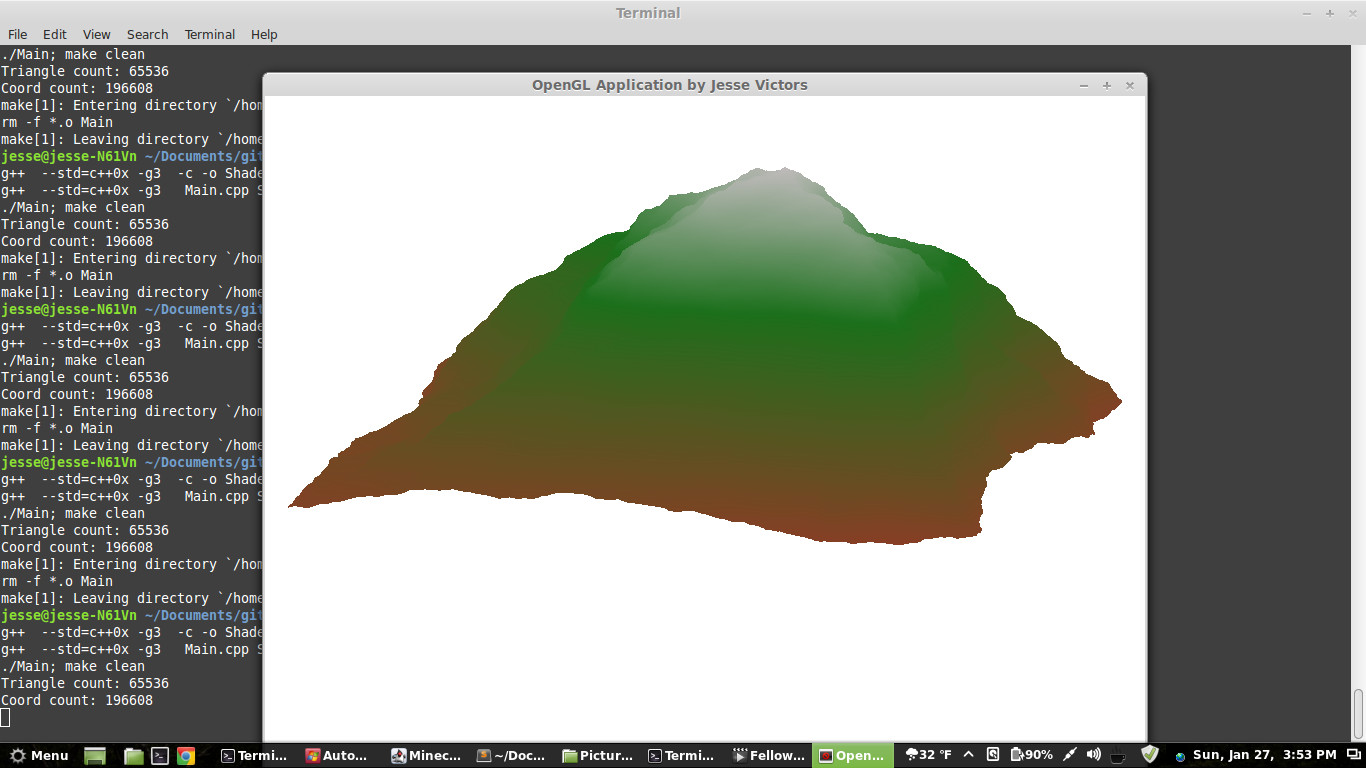
\includegraphics[width=80mm]{resources/Sierpinski_Mountain.jpg}
		\caption{My original Sierpinski Mountain.}
	\end{minipage}
}
\end{figure}

In this initial framework, I had a World class, which held various Models. A Model was an abstract class because it contained pure virtual functions, which were defined in subclasses, such as a MandelModel and a GroundModel.

\section{Git}

Git is a brilliant distributed revision control and source-code management system, and makes it exceptionally easy to branch, merge, and navigating changes. Git is also very amendable to distributed development of a large project. However, in this project I primarily used Git to assist me with developing my framework.

One of my main goals was focused responsibility and separation of dependencies.

\section{Development}

\begin{figure}[htbp]
\centering
\fbox
{
	\begin{minipage}{8 cm}
		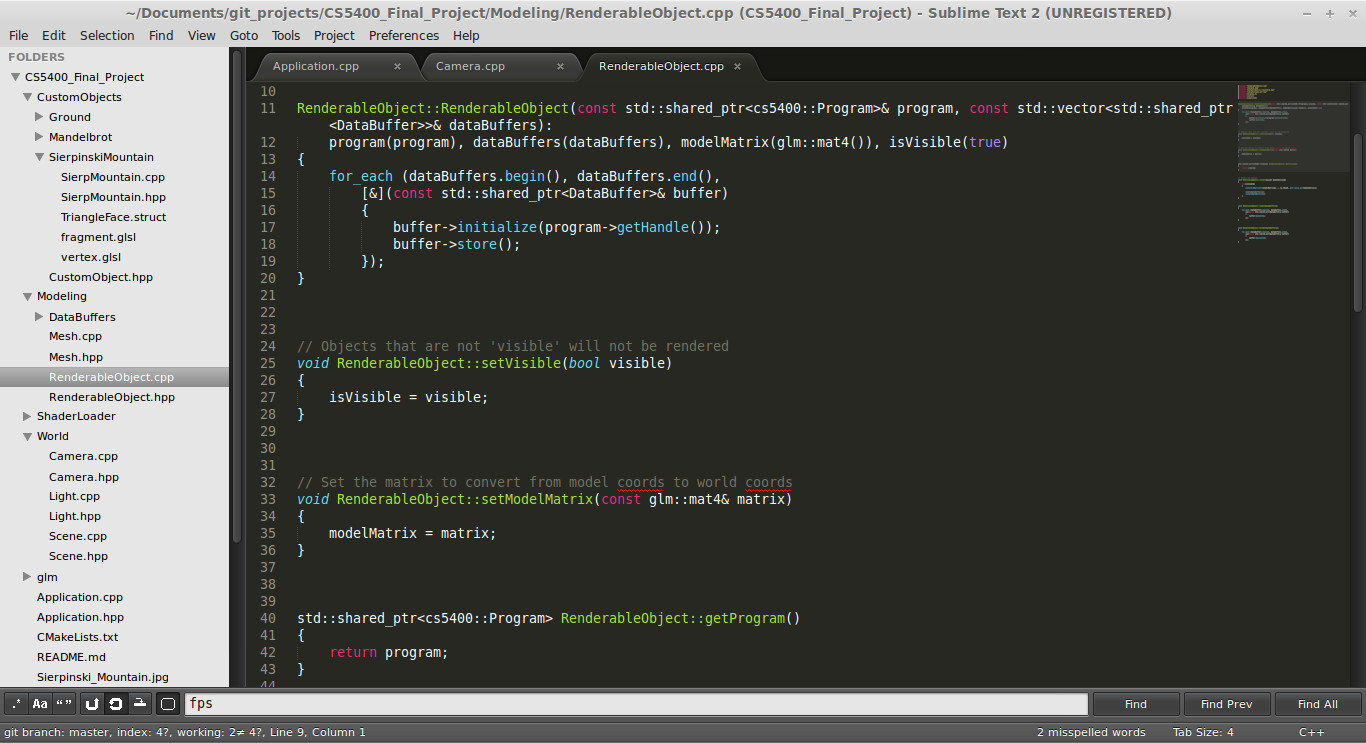
\includegraphics[width=80mm]{resources/editing_in_sublime.png}
		\caption{Sublime Text 2 was my primary text editor. I compiled in the command-line.}
	\end{minipage}
}
\end{figure}

I developed all of my graphics assignments in Linux Mint 14. I used the Sublime Text editor, and command-line.

\section{CMake}

\section{Visual Results}

Visually, I have a scene containing four models: a large square representing the ground, two artificially- and randomly- generated mountains, and a three-dimensional spiral that is textured using the Mandelbrot fractal.

\subsubsection{Ground} test

\begin{figure}[htbp]
\centering
\fbox
{
	\begin{minipage}{8 cm}
		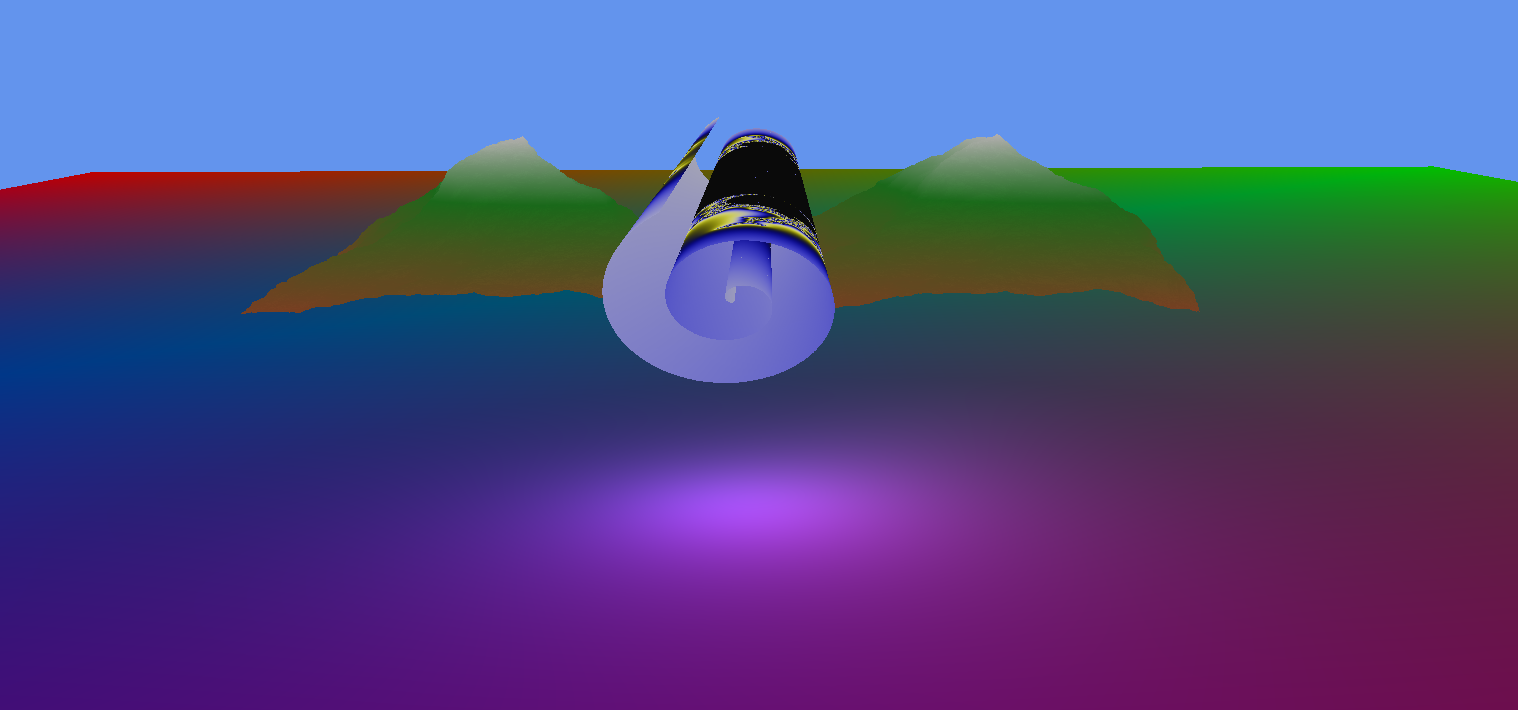
\includegraphics[width=80mm]{resources/screenshot1.png}
		\caption{Each corner of the ground is assigned a color, with red assigned twice (to opposite corners). The colors are then blended.}
	\end{minipage}
}
\end{figure}

The ground is a simple 2D square. It is constructed to be a 1-by-1 square consisting of two triangles, but the Application::addGround method transforms it to a 2-by-2 matrix using a GLM scaling matrix. Coloring is done in the shaders. The vertex shader detects what corner it is dealing with, and assigns a solid RGB color accordingly, which is then passed to the fragment shaders via a varying data type. This color is blended across the triangles in the graphics card, and the fragment shader picks this up and uses it as the main color for that fragment. Ambient and specular lighting is further applied to generate the final color for the particular pixel.

\subsubsection{3D Mountains}

\begin{figure}[htbp]
\centering
\fbox
{
	\begin{minipage}{8 cm}
		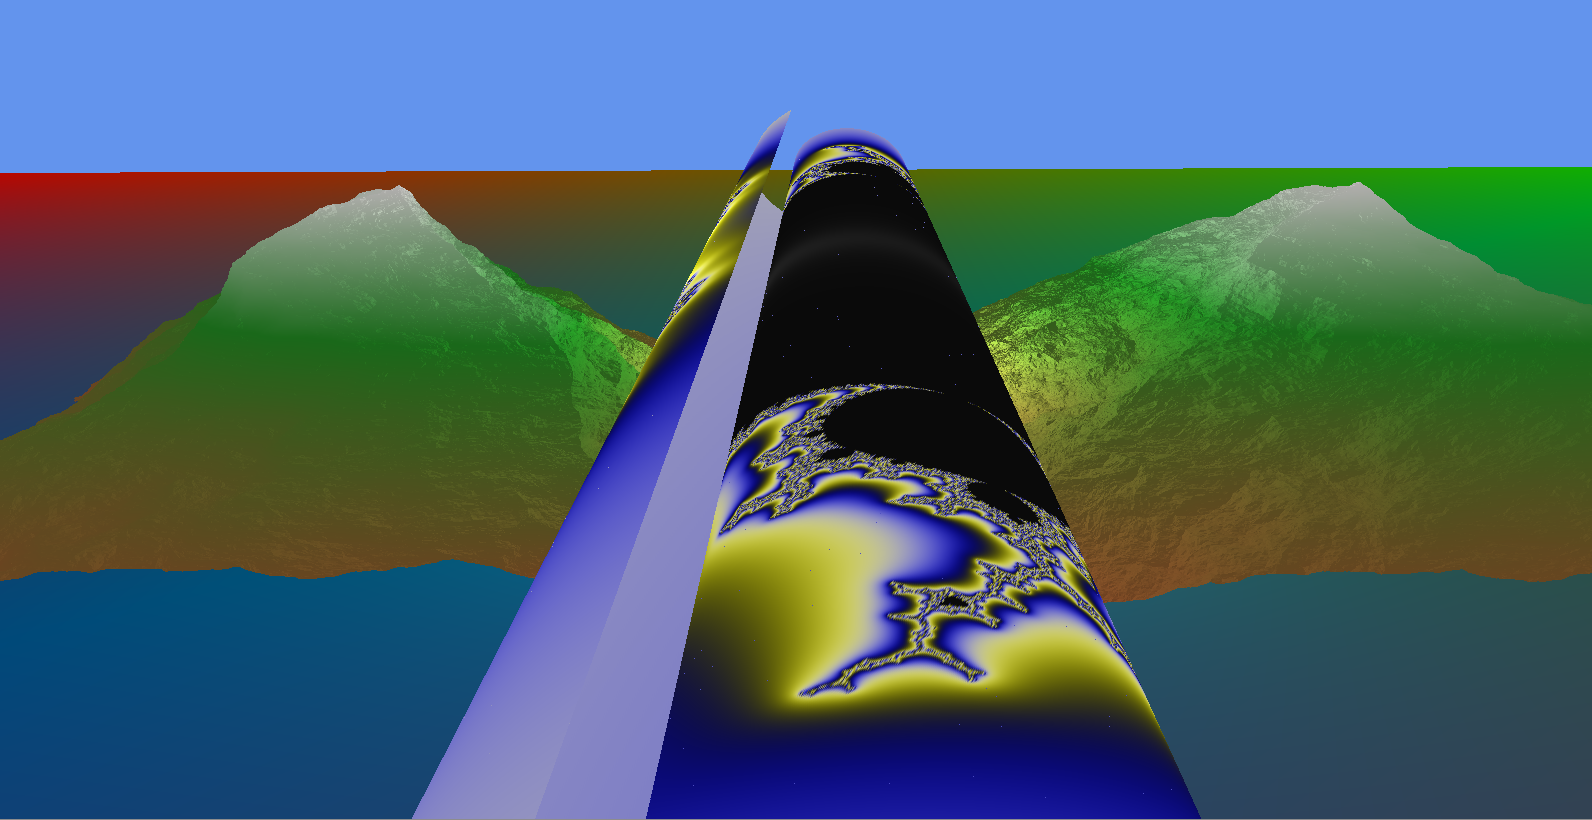
\includegraphics[width=80mm]{resources/screenshot2.png}
		\caption{The 3D spiral is centered in between two artificially-generated snow-capped mountains.}
	\end{minipage}
}
\end{figure}

The scene contains two artificially-generated mountains. As with all the other models, the data is set up on the CPU side and passed to the GPU for rendering. The generation algorithm starts a basic pyramid shape. Four triangles meet at the top, connect at a central top, and form a square at the bottom. A modified form of the Sierpinski Gasket algorithm is then used to generate the mountain. Each triangle is subdivided into four equally-sized sub-triangles. This involves finding the midpoint in the side of the main triangle. If the triangle face was recursively subdivided N levels deep, there would basically no difference in the appearance, as it would still look like a flat triangle. However, if an randomized offset is added after the midpoint is found, a level of randomness can be added. By making the magnitude of the random offset poportional to the length of the triangle leg, there are big changes at first, and as the recursion gets deeper, smaller and smaller offset are added. This results in a lightly rough surface which contains fine details.

I used the Mersenne Twister pseudo random number generator for generating the random offset. This generator produces high quality random numbers at high speed, and is built into the C++ STL. I will strive to use this algorithm for any future for applications which need random numbers. It is far superior to the Linear Congruent Generator used in many simple applications.

Better mountains could have been produced using Perlin noise. With Perlin noise, values at points far away from each other are essentially uncorrelated and are random, but values at points close to each other are highly likely to be similar to one another. For example, a point that becomes the top of a hill or mountain is at a value random from far-away points on a landscape, but points closer will be of a similar height. This produces rounded and smooth-looking terrain. The downside of the Sierpinski Gasket algorithm is that the mountain still looks roughly like a pyramid. From above or below, it's obvious that it has square base. This could be partially resolved by changing from a four-sided base to a 5-, 6-, or even 7- sided base. Perlin noise would still be a better and more efficient choice however, but the mountains look pretty decent just as they are.

\subsubsection{Mandlebrot Fractal on a 3D spiral}

\begin{figure}[htbp]
\centering
\fbox
{
	\begin{minipage}{8 cm}
		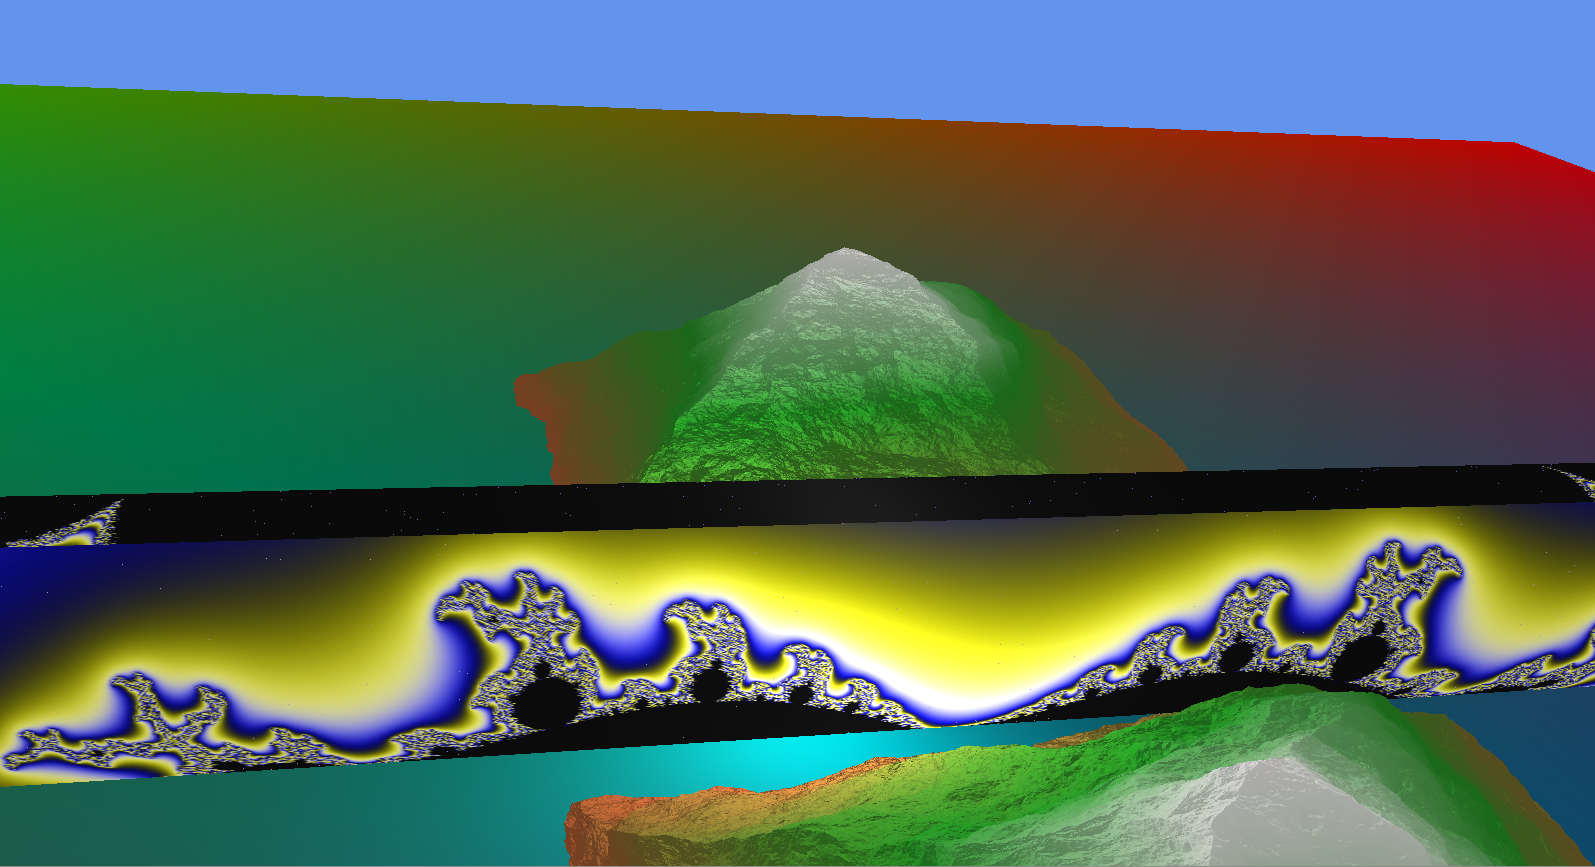
\includegraphics[width=80mm]{resources/screenshot3.png}
		\caption{The end of the fractal reaches right to the end of the spiral. Figure 2 also illustrates the fractal wrapping around one side of the spiral.}
	\end{minipage}
}
\end{figure}

\subsection{Limitations}

\subsubsection{Lack of support for hierarchical modeling}

My framework does not currently support hierarchical modeling, which is used for animating a large composite object by subdividing it into many smaller pieces. This process involves \textit{boning} (sometimes known as \textit{rigging}) where the object is modeled using a set of bones. Each bone its own matrix for a three-dimensional transformation, such as position, scaling, and orientation, in addition to a reference to its parent and any children. Boning is useful because the programmer or animator does not have to worry about the positioning and orientation of every individual piece of the overall object, rather each piece knows where it should belong relative to its neighbors in the hierarchicy. Thus, the whole model can be rotated or translated, and all the various components will be appropriately transformed.

Boning only produces a thin skeleton of the model, and is typically not sufficient for a full model of the object, and certainly not for animation. The next step in hierarchical modeling involves \textit{skinning}, where a mesh is laid on top of the bones. A simple skin might be a rectangular prism or a cylinder, centered and oriented on the underlying bone. The skin is typically a mesh of vertices. If the model was of a human being, this mesh could be rounded, bulged in the middle, and laid over the humerus bone to model the upper arm.

In order to support the boning and skinning elements of hierarchical modeling, the framework would have to include a tree-like structure for boning. Each bone would need references to other bones, its transformation matrix, and its appropriate skin. Each skin would likely have its own texture, index, and texture buffers. This would require a significant refactoring of my framework, as the RanderableModel has its own data buffers and knows how to render itself. To support hierarchical modeling, the RenderableObject would need to keep track of a root bone (from which all other bones are descendants) and only the skin would know how to render itself. In addition, in order to support any type of animation, I'd have to be able to access the appropriate bones and pivot them (thus modeling joints) accordingly.

One of the problems with simplistic hierarchical modeling is that 1) there can be visible gaps in the joints between bones,  caused by the skin of one bone visually seperating from the skin of another bone; and 2) the skin is inflexible, resulting in a movement looking robotic. Both of these can be fixed by having the points of the skin link to one another, and possible the points of neighboring skins. Then the skin mesh has to flex and move in accordance with the changes of the bones. This becomes very complex, as each point on the mesh has to translate itself relative to its neighboring points. This could be performed using force fields in physics, or using energy functions. If done correctly, the result can be impressive and highly realistic animation. The downside is that the code becomes much more complex, and there's a significant increase of the computations required on the CPU, the GPU, and the data transfer through the system bus.

\subsubsection{Inefficiencies}

One of the disadvantages of my code is its inefficiencies, which become more obvious when the detail is turned up and the program is executed on slower hardware, such as a Nvidia GT 240m (released November 2009).

too many verticies for spiral, rendered even if offscreen

\subsubsection{Incompleteness}



\subsubsection{Repetition of shader code}



\section{Conclusion}
Write your conclusion here.

\LaTeX{}

\end{document}
